% ==============================================================================================
%  ____        _ _     _               ____  ___ ____ _   _                                
% | __ ) _   _(_) | __| | ___ _ __    |  _ \|_ _/ ___| | | |    _   _ ___  __ _  __ _  ___ 
% |  _ \| | | | | |/ _` |/ _ \ '__|   | |_) || | |   | |_| |   | | | / __|/ _` |/ _` |/ _ \
% | |_) | |_| | | | (_| |  __/ |      |  _ < | | |___|  _  |   | |_| \__ \ (_| | (_| |  __/
% |____/ \__,_|_|_|\__,_|\___|_|      |_| \_\___\____|_| |_|    \__,_|___/\__,_|\__, |\___|
%                                                                               |___/      
% ==============================================================================================

\section{Применение ``CATIA-GDML geometry builder'' к CBM RICH}\label{sec:secBuilderCbmRich}

Значительная часть работы над ``Builder'' выполнялась при поддержке группы CBM RICH, поэтому самая сложная MC-модель, построенная с помощью ``Builder'', это CBM RICH. Модель была построена за несколько итераций, имеет достаточно сложную иерархию и характеризуется высокой степенью подробностей.
Геометрическая MC-модель детектора RICH эксперимента CBM имеет многоуровневую структуру, в основном обоснованную физической структурой сборки, но иногда и \todo бывает неочевидной и неестественной с целью повышения эффективности проведения частиц.
Для моделирования эксперимента в CBM используется пакет CbmRoot. Для того, чтобы GDML файлы, экспортированные из CATIA, корректно читались CbmRoot было написано дополнение, описанное в секции~\ref{sec:secFairModule}.

На момент написания данной работы инженерный проект не был завершён --- некоторые узлы были проработаны достаточно подробно и прошли несколько этапов уточнения, в которых модель менялась принципиально. В то же время некоторые узлы существуют лишь на концептуальном уровне. В первую очередь к ним относится форма и конструкция корпуса детектора, проектирование которой является относительно несложной задачей и может быль отложено на более поздний этап. Большая часть корпуса не оказывает влияния на эффективность детектора, т.к. лежит за пределами геометрического аксептанса, поэтому допускается моделирование физики детектора с упрощённой моделью корпуса, либо вообще без него.

В детекторе RICH можно выделить несколько подсистем --- фоточувствительная камера, магнитный экран вокруг камеры, зеркала, система опор зеркал, часть ионопровода в RICH, корпус детектора. Рассмотрим реализацию каждой подсистемы в MC-модели, построенной с помощью ``CATIA-GDML geometry builder''.

% ==============================================================================================
%  __  __ _                         
% |  \/  (_)_ __ _ __ ___  _ __ ___ 
% | |\/| | | '__| '__/ _ \| '__/ __|
% | |  | | | |  | | | (_) | |  \__ \
% |_|  |_|_|_|  |_|  \___/|_|  |___/
%                                   
% ==============================================================================================

\subsection{Фокусирующая система --- сферические зеркала}\label{sec:secRICHgeoMirror}

% subsubsection ->textbf
%\label{sec:secRICHgeoMirrorMis}

\textbf{MC-геометрия фокусирующей системы с возможностью задания индивидуальных отклонений}

Для отладки методов калибровки положения зеркал необходимо выполнять моделирование с геометрией, имеющей отклонения сегментов зеркал, заданные определённым образом. Техника \todo CLAM разработана с расчётом на то что отклонение каждого сегмента может быть получено в результате двух вращений. Если для каждого сегмента зеркала ввести фиксированный центр и локальную систему координат с осями $\overrightarrow{n}$, $\overrightarrow{\tau}$ и $\overrightarrow{b}$, то вращение должно осуществляться последовательно вокруг \todo.

Для того, чтобы это было возможно в разработанной MC-модели CBM RICH потребовалось ввести два промежуточных уровня вложенности --- один для каждого типа зеркал и ещё один для каждого сегмента. Первый промежуточный уровень вложенности переносит центр сегмента в начало координат. Второй обеспечивает вращение вокруг оси \todo. При позиционировании в газ вводится отклонение вокруг второй оси \todo.

\todo \textbf{уточнить}

Одна из задач, которую приходится решать с описываемой геометрией --- выполнять многократно моделирование прохождения частиц с разными значениями отклонения сегментов зеркал. Это означает, что пользователь должен иметь возможность легко модифицировать геометрию. По этой причине значения отклонений каждго сегмента зеркала были вынесены в качестве параметров модели, что выглядит как список из 160 параметров в <define> секции GDML файла. Имя каждого параметра построено по правилу ``misalign\textunderscore AXIS\textunderscore A\textunderscore B'', где AXIS --- осьвращения --- либо ``x'', либо ``y'', $A \in [0,7]$ --- номер сегмента вдоль вертикального направления, а $B \in [0,9]$ --- номер сегмента вдоль горизонтального направления.

\todo \textbf{картинка с нумерации сегментов зеркал}

В итоге получается две модели RICH --- одна для общего пользования с идеально позиционированными зеркалами и вторая отдельно для отладки методов коррекции положения зеркал. Для того, чтобы не \todo плодить сущности без необходимости оба зеркала смоделированы в одной CATIA сборке, а разделение на два GDML файла выполняется путём комментирования некоторых частей одного GDML файла, экспортируемого из CATIA. Использование геометрии с индивидуальным отклонениями зеркал для моделирования в общей установке CBM не рационально, т.к. в такой геометрии больше объёмов. Кроме того, в геометрии с отклонениями зеркал по запросу пользователя были выключены некоторые подробности (такие как, например, каркас детектора и опоры зеркал), т.к. они не оказывают никакого влияния на исследование CLAM, но замедляют моделирование.

% ==============================================================================================
%  __  __                        _   _                                       
% |  \/  | __ _  __ _ _ __   ___| |_(_) ___     ___  ___ _ __ ___  ___ _ __  
% | |\/| |/ _` |/ _` | '_ \ / _ \ __| |/ __|   / __|/ __| '__/ _ \/ _ \ '_ \ 
% | |  | | (_| | (_| | | | |  __/ |_| | (__    \__ \ (__| | |  __/  __/ | | |
% |_|  |_|\__,_|\__, |_| |_|\___|\__|_|\___|   |___/\___|_|  \___|\___|_| |_|
%               |___/                                                        
% ==============================================================================================

\subsection{Магнитный экран}\label{sec:secRICHmagScreen}

% Три различные системы для разных задач
Для выполнения геометрического моделирования применялась САПР CATIA~v5, расчёт распределения паразитного магнитного поля внутри экрана выполнялся с помощью МКЭ в OPERA3d/TOSCA, а моделирование прохождения частиц в условиях пучка выполнялось в CbmRoot.

% \todo проверить ссылку

\begin{figure}[H]
\centering
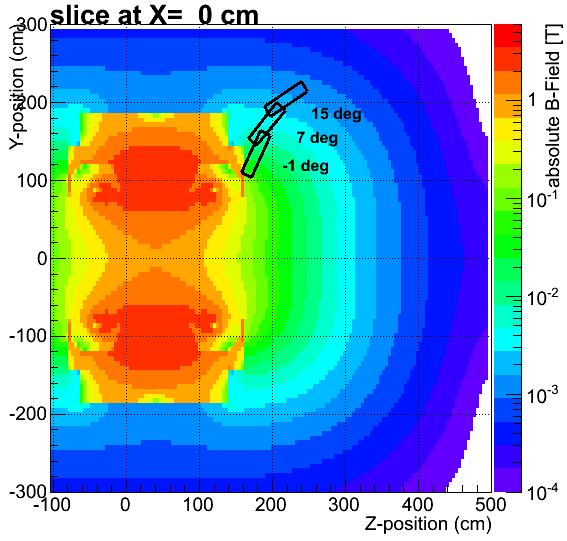
\includegraphics[width=0.5\textwidth]{pictures/MagScreenPositions.png}
\caption{Варианты расположения фоточувствительной камеры CBM RICH в магнитном поле в зависимоти от угла наклона фокусирующих зеркал~\cite{RichCameraInField}.}
\label{fig:MagScreenPositions}
\end{figure}

% ==============================================================================================
%  __  __                        _   _           __ _      _     _ 
% |  \/  | __ _  __ _ _ __   ___| |_(_) ___     / _(_) ___| | __| |
% | |\/| |/ _` |/ _` | '_ \ / _ \ __| |/ __|   | |_| |/ _ \ |/ _` |
% | |  | | (_| | (_| | | | |  __/ |_| | (__    |  _| |  __/ | (_| |
% |_|  |_|\__,_|\__, |_| |_|\___|\__|_|\___|   |_| |_|\___|_|\__,_|
%               |___/                                              
% ==============================================================================================

\subsubsection{Магнитное поле в области фоточувствительной камеры}\label{sec:CbmRichMagField}

\todo \textbf{Да, здесь наблюдается некоторое дублирование мыслей и расхождение цифр, собранных их двух источников. Нужно как-то это дело причесать.}

Моделирование распределения магнитного поля, созданного дипольным магнитом, с помошью пакета OPERA3d/TOSCA показало, что фоточувствительная камера расположена в области, где паразитное поле составляет 10--50~мТл. Измерения показали, что для планируемой модели МА~ФЭУ эффективность регистрации одиночных фотонов значительно падает, если поле превышает уровень 1--2~мТл. Таким образом, магнитное поле в области фотосенсоров должно быть опущено до допустимого уровня.

% According to TOSCA$^3$ calculations, the photon camera is exposed to significant magnetic stray fields in the order of 10~mT to 50~mT. Measurements show that the single photon detection efficiency of the foreseen MAPMTs drops significantly for values exceeding 1~mT to 2~mT especially in the edge and corner pixels [6]. Therefore, the magnetic field strength in the region of the photon sensors has to be kept below this value.

Есть два способа уменьшить поле в области камеры --- повернуть зеркало и, следовательно, отодвинуть камеру от магнита, и поставить магнитный экран вокруг камеры. В CBM RICH была проведена оптимизация угла наклона зеркала точки зрения эффективности реконструкции и было решено спроектировать магнитный экран вокруг камеры.
% Есть также третий вариант, который заключается во введении дополнительного отражения на пути черенковских фотонов. Этот подход, однако, был исключён, т.к. дополнительное отражение приводит к увеличению необходимой светочувствительной плоскости, а это значительно увеличивает стоимость детектора.

% In order to cope with the magnetic stray field in the region of the photon camera, two design options are considered and currently studied. The first option is to rotate the two mirror planes and to move the camera modules further away from the beam axis where the magnetic stray field is lower. In addition, a shielding box enfolding the camera modules can reduce the magnetic field strength in the region of the photocathodes significantly. The second option is the use of a second mirror reflecting the Cherenkov photons to the camera positioned farther away from the magnet. This option, however, requires a larger camera surface due to an increased focal length. Details on all design options can be found in [6].

% Ссылка на прогресс репорт 2015 стр. 53.

Положение фоточувствительной камеры в пространстве определяется относительно зеркал исходя из соображений эффективности регистрации колец. В CBM детектор RICH расположен непосредственно за дипольным магнитом, причём отражённые от сферических зеркал черенковские фотоны летят в направлении противоположном пучку. Уменьшение угла наклона зеркал теоретически приводит к повышению эффективности детектора, но на практике невозможно из-за нехватки пространства для размещения камеры в небольшом зазоре между магнитом и конусом аксептанса RICH. Увеличение угла наклона зеркал позволило бы вывести фотодетектор далее вверх из области магнитного поля, но это приводит к нежелательным оптическим эффектам, отрицательно влияющим на эффективность. Следовательно, камера должна быть расположена очень близко к дипольному магниту. Отсюда возникает необходимость экранировать камеру от магнитного поля, составляющего 50-100~мТл в области МА~ФЭУ. Рассчитано, что данное семейство МА~ФЭУ может работать в магнитном поле до 1~мТл без снижения эффективности.

% ==============================================================================================
%  __  __                        _   _                                       
% |  \/  | __ _  __ _ _ __   ___| |_(_) ___     ___  ___ _ __ ___  ___ _ __  
% | |\/| |/ _` |/ _` | '_ \ / _ \ __| |/ __|   / __|/ __| '__/ _ \/ _ \ '_ \ 
% | |  | | (_| | (_| | | | |  __/ |_| | (__    \__ \ (__| | |  __/  __/ | | |
% |_|  |_|\__,_|\__, |_| |_|\___|\__|_|\___|   |___/\___|_|  \___|\___|_| |_|
%               |___/                                                        
% ==============================================================================================

\subsubsection{Магнитный экран вокруг камеры}\label{sec:secCbmRichCameraShield}

Т.к. рассматривалось два варианта форм фоточувствительной камеры --- четыре плоскости и два цилиндра --- потребовалось прорабатывать два варианта формы магнитного экрана. На \figref{fig:ShieldingBox} показан чертёж первого рассчитанного магнитного экрана для плоского варианта камеры, а на \figref{fig:ShieldingBoxMC} --- первая версия магнитного экрана в CbmRoot.

\begin{figure}[H]
\centering
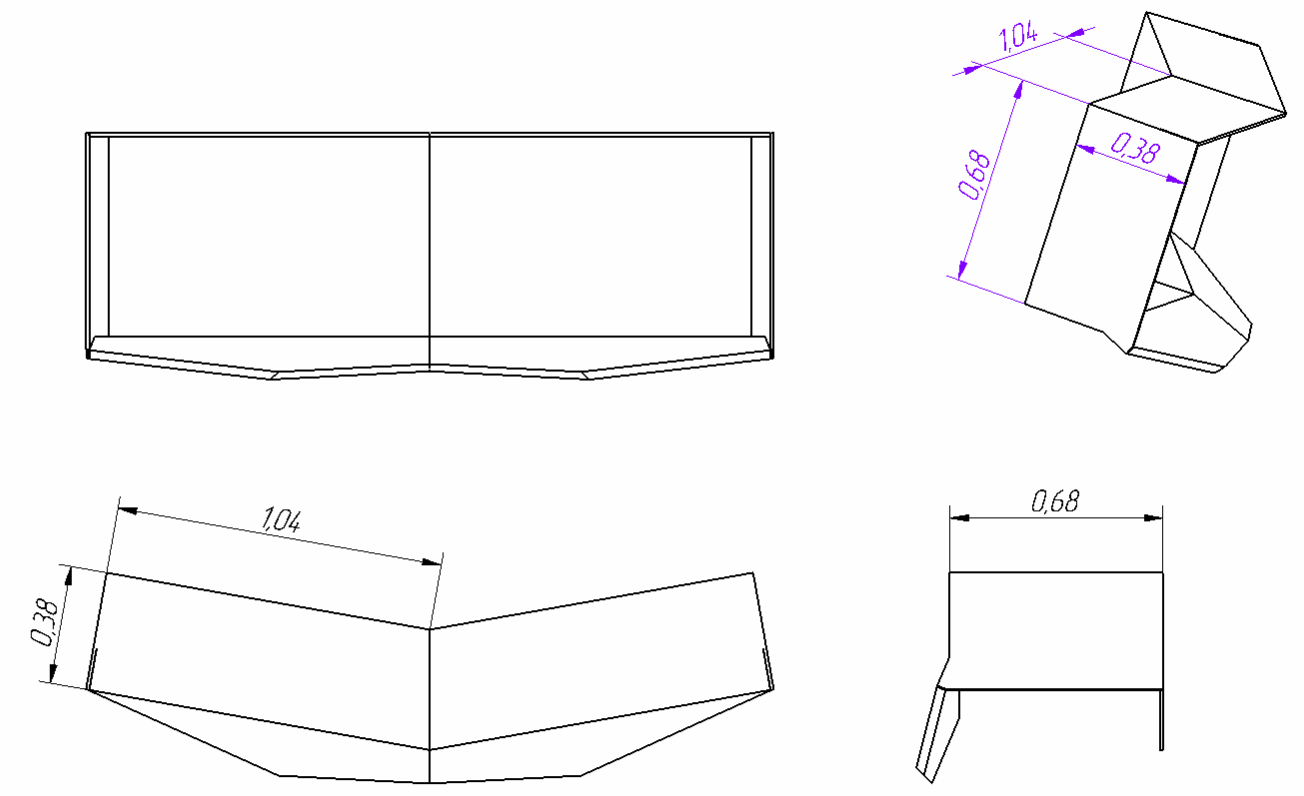
\includegraphics[width=0.7\textwidth]{pictures/First_shielding_box_1.png}
\caption{Первый эскизный проект магнитного экрана.}
\label{fig:ShieldingBox}
\end{figure}

\begin{figure}[H]
\begin{minipage}[b]{0.495\textwidth}
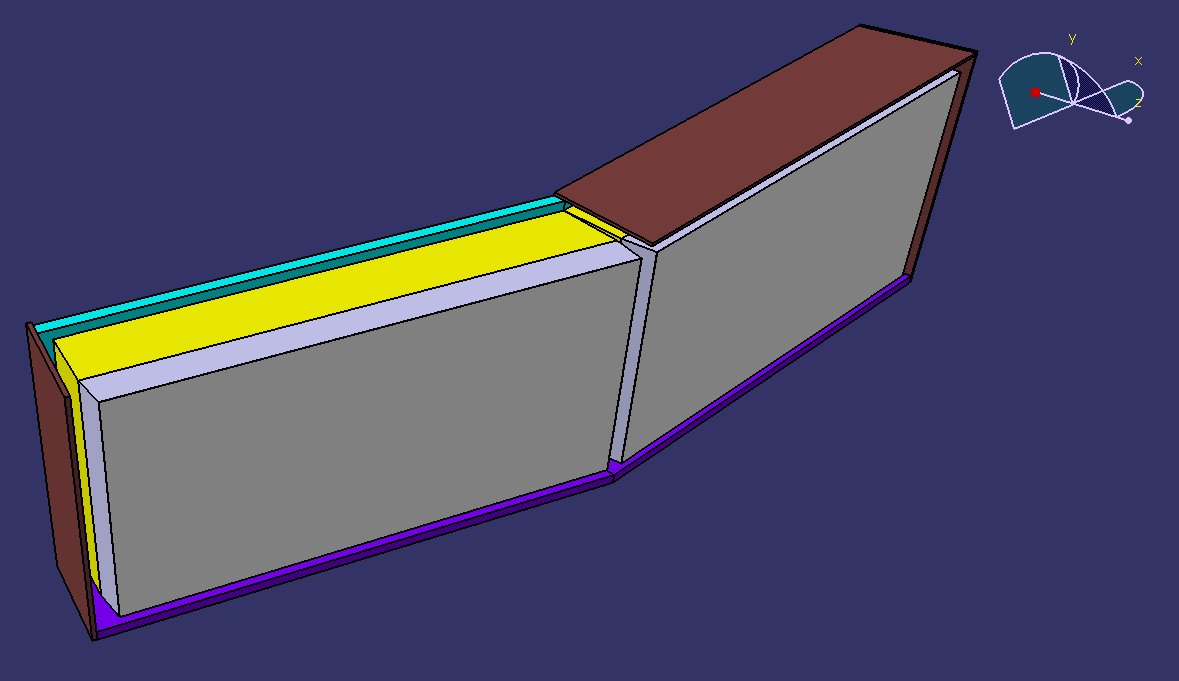
\includegraphics[width=1.0\textwidth]{pictures/ShieldingBox_MC.png}
\end{minipage}
\hspace{0.01\textwidth}
\begin{minipage}[b]{0.495\textwidth}
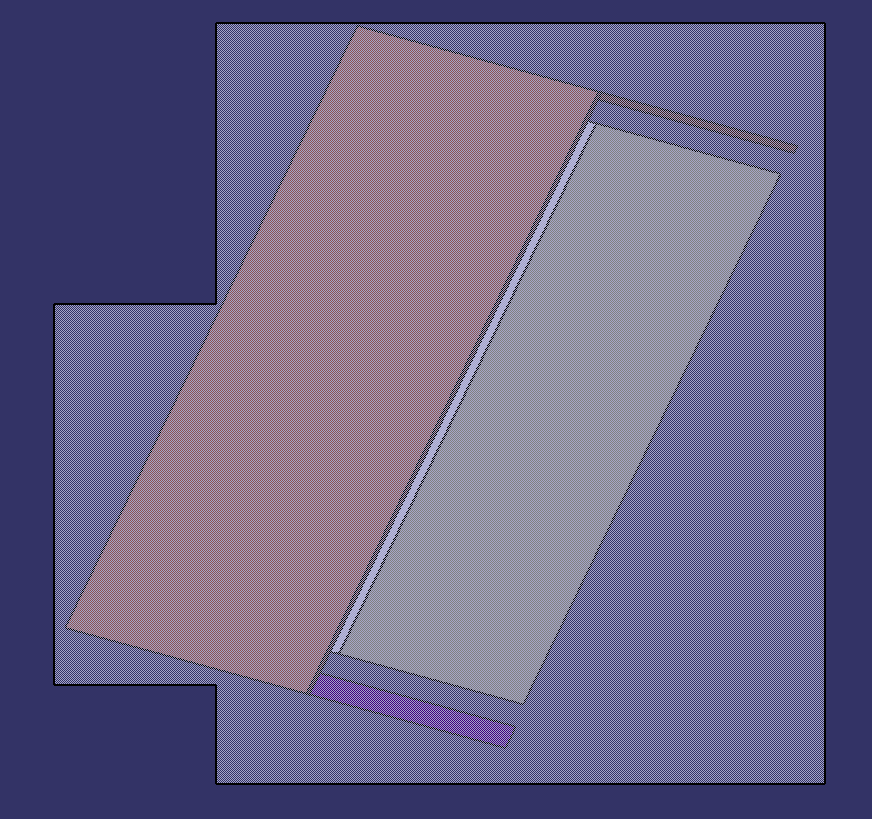
\includegraphics[width=0.7\textwidth]{pictures/ShieldingBox_MC2.png}
\end{minipage}
\caption{Первая версия магнитного экрана в CbmRoot. Серым цветом показаны МА~ФЭУ, жёлтым --- электроника.}
\label{fig:ShieldingBoxMC}
\end{figure}

На момент написания данной работы проект магнитного экрана не был завершён, однако было выполнено эскизное проектирование и моделирование распределения магнитного поля в пакете OPERA3d/TOSCA. Было определено, что магнитный экран должен иметь нижнюю и заднюю (ближную к магниту) стенку толщиной 30~мм, а остальные --- толщиной 10~мм. Одной из проблем при проектировании магнитного экрана является задача минимизации массы; т.к. экран должен быть выполнен из материала с высоким коэффициентом магнитной проницаемости, лёгкие металлы типа алюминия не подходят. Масса каждого из двух экранов получилась равна 850~кг. В экране присутствуют отверстия необходимые для отвода кабелей и для обеспечения охлаждения.

% \todo
% Порассуждать о клюве (язычке)
Для обеспечения высокого потока линий магнитного поля у магнитного экрана со стороны пучка предусмотрено утолщение. Геометрически оно ограничено аксептансом, а со стороны здравого смысла --- габаритами и массой.

% ==============================================================================================
%   ____                               
%  / ___|__ _ _ __ ___   ___ _ __ __ _ 
% | |   / _` | '_ ` _ \ / _ \ '__/ _` |
% | |__| (_| | | | | | |  __/ | | (_| |
%  \____\__,_|_| |_| |_|\___|_|  \__,_|
%                                      
% ==============================================================================================

\subsection{Фоточувствительная камера}\label{sec:secRICHgeoCamera}

Планируется, что фоточувствительная камера CBM RICH будет составлена из модулей, содержащих 2$\times$3 МА~ФЭУ, см. \figref{fig:H12700drawing}. Один такой МА~ФЭУ имеет габариты 52$\times$52~мм$^2$, между МА~ФЭУ оставляется зазор 1~мм для запаса по точности, таким образом размер модуля составляет 158мм$\times$105мм.

\begin{figure}[H]
\centering
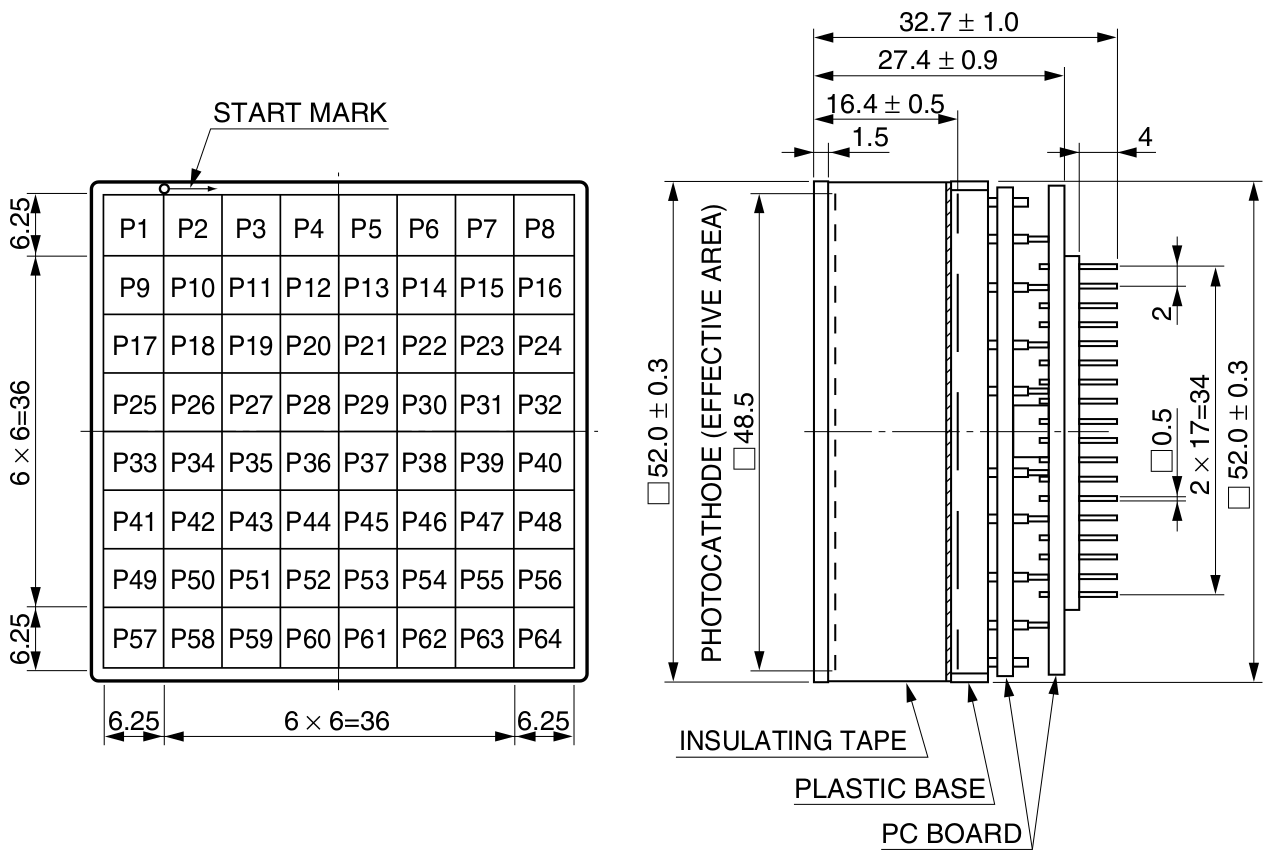
\includegraphics[width=0.7\textwidth]{pictures/H12700_drawing.png}
\caption{Чертёж МА~ФЭУ H12700 из документации.}
\label{fig:H12700drawing}
\end{figure}

\begin{figure}[H]
\begin{minipage}[b]{0.495\textwidth}
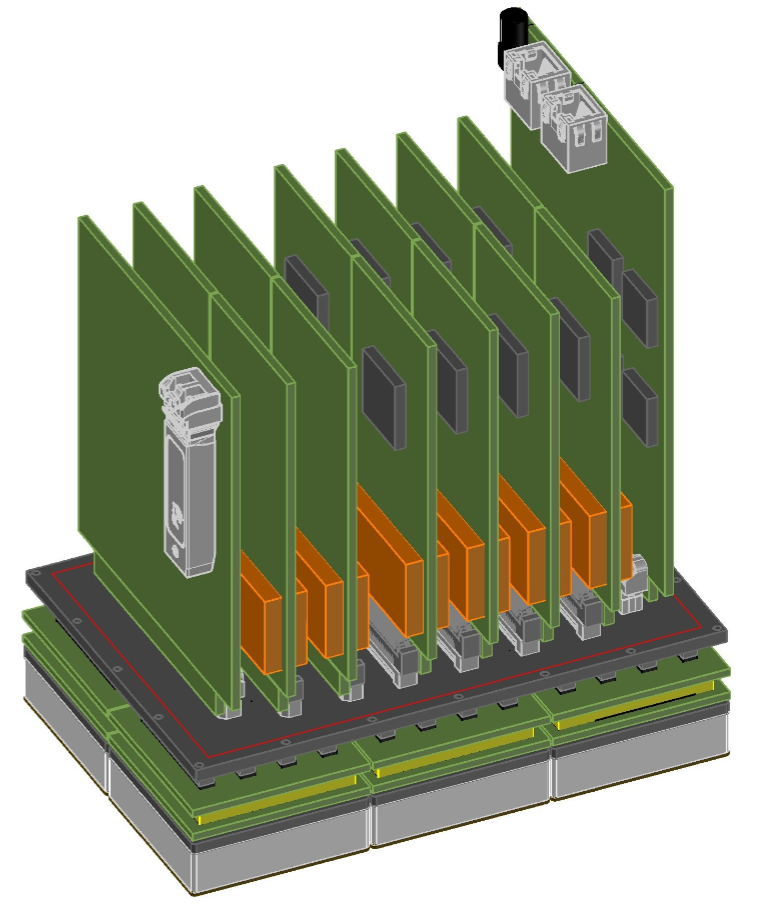
\includegraphics[width=1.0\textwidth]{pictures/PMTmoduleCAD.png}
\end{minipage}
\hspace{0.01\textwidth}
\begin{minipage}[b]{0.495\textwidth}
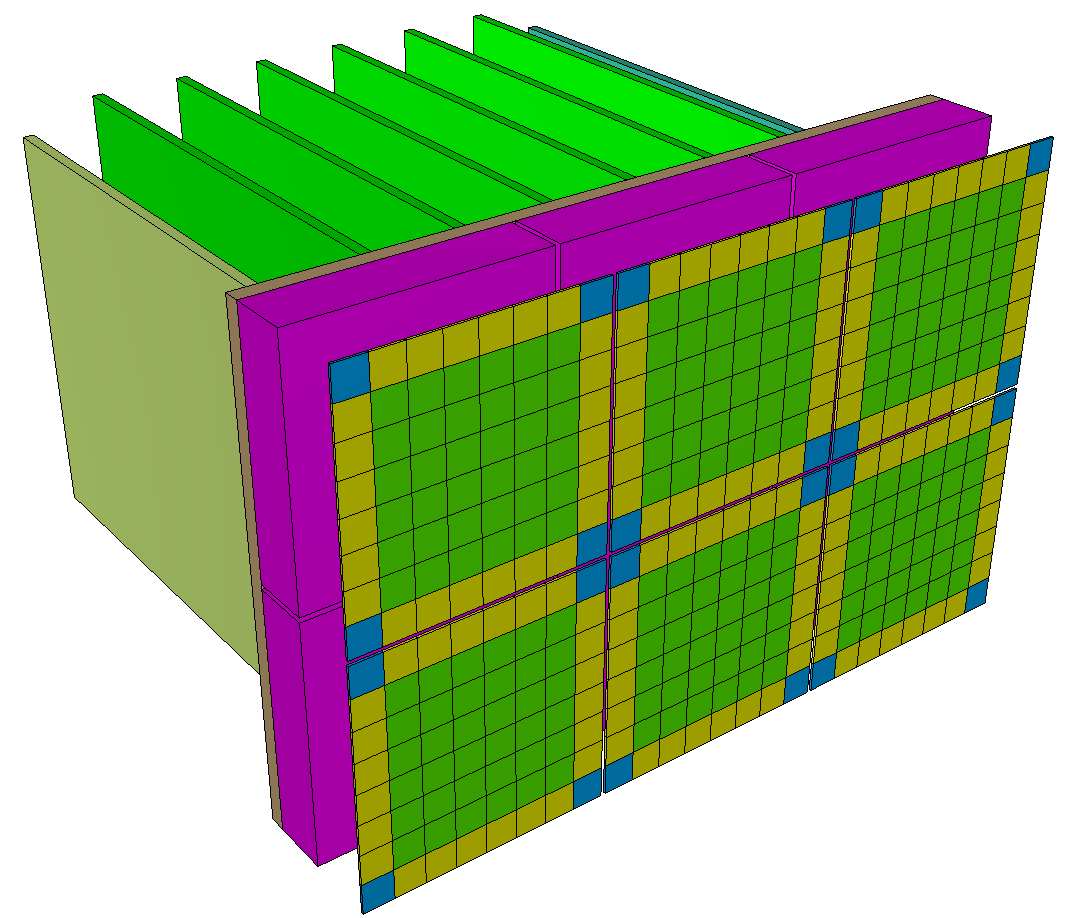
\includegraphics[width=1.0\textwidth]{pictures/Module_1_cut.png}
\end{minipage}
\caption{CAD-модель (слева) и MC-модель (справа) модуля фоточувствительной камеры CBM RICH.}
\label{fig:geoMCmodule}
\end{figure}

Иерархия объёмов, моделирующих модуль фоточувствительной камеры CBM RICH приведена на \figref{fig:Module_geoStructure}.

\begin{figure}[H]
\centering
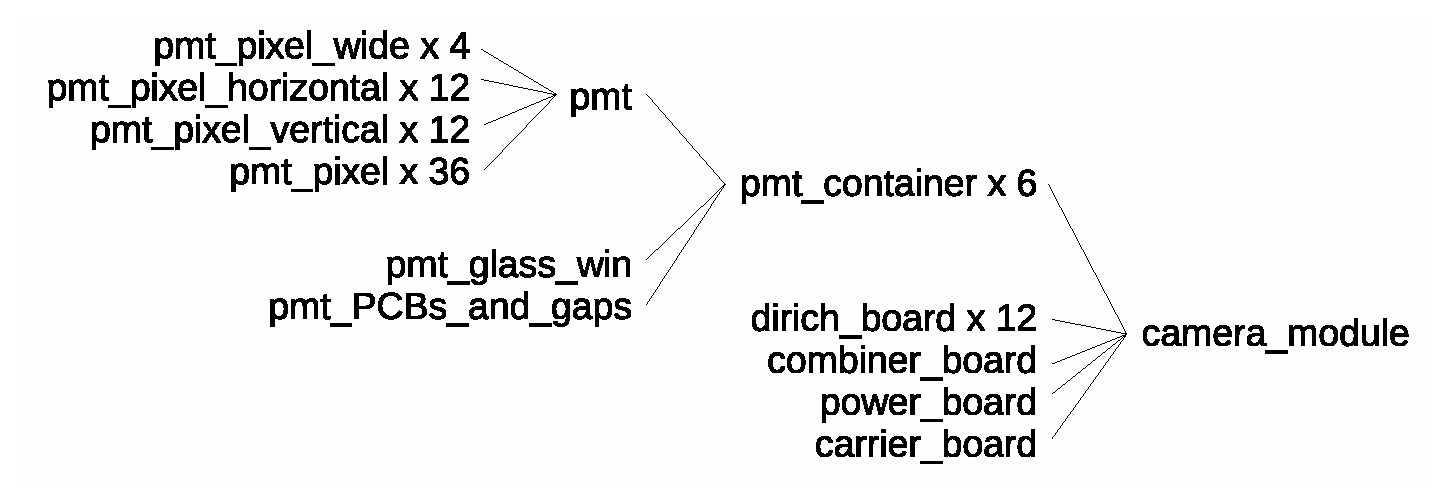
\includegraphics[width=0.7\textwidth]{pictures/Module_geoStructure.eps}
\caption{Иерархия объёмов, моделирующих модуль фоточувствительной камеры CBM RICH.}
\label{fig:Module_geoStructure}
\end{figure}

%Пиксели
%№№ 2-7, 58-63, 9, 17,..., 49, 16, 24,..., 56
МА~ФЭУ моделируется до уровня пикселей. Это позволяет максимально приблизить моделирование прохождения частиц в CbmRoot и обработку реальных данных. В соответствии с документацией, у МА~ФЭУ H12700 пиксели имеют разные размеры (см. \figref{fig:H12700drawing}): угловые пиксели (№№ 1, 8, 57, 64) 6.25мм$\times$6.25мм, пиксели по краям, кроме угловых, --- 6.25мм$\times$6мм, остальные, центральные пиксели --- 6мм$\times$6мм. Для того, чтобы представить три типа пикселей в MC-модели, необходимо три отдельных объёма, имеющих разную форму. Чтобы сделать модель максимально понятной и гибкой принято решение отделить пиксели из крайних горизонтальных рядов от пикселей из крайних вертикальных рядов и моделировать их с помощью двух разных объёмов размером 6мм$\times$6.25мм и 6.25мм$\times$6мм соответственно. Это позволит позиционировать все пиксели без поворотов.

Таким образом вводится 4~объёма:
\begin{itemize}
\itemsep0pt
\item \volumename{pmt\textunderscore pixel\textunderscore wide} для угловых пикселей,
\item \volumename{pmt\textunderscore pixel\textunderscore horizontal} для пикселей в крайних горизонтальных рядах,
\item \volumename{pmt\textunderscore pixel\textunderscore vertical} для пикселей в крайних вертикальных рядах и
\item \volumename{pmt\textunderscore pixel} для всех остальных пикселей, расположенных в центральной зоне.
\end{itemize}
Все 4 объёма имеют форму примитива box с толщиной вдоль оси Z, равной 0.5мм, материал CsI, который в данный момент используется в моделировании как активный материал для фоточувствительных элементов. Толщина выбрана произвольно, она не имеет значения, т.к. из-за того, что материал объёма активный, т.е. объём объявлен чувствительным, система проведения частиц будет вырабатывать сигнал о пересечении треком границы объёма и передавать управление методу \methodname{ProcessHits} класса детектора \classname{CbmRich}. В реализации этого метода вырабатывается Point, причём физика не оказывает никакого влияния. Даже если толщина объёма слишком маленькая, чтобы произошло какое-либо взаимодействие, флаг активности обязывает систему вызвать \methodname{ProcessHits}.

Объём \volumename{pmt} соответствует части МА~ФЭУ, включающей в себя фотокатод (пиксели) и динодную систему, и имеет толщину $16.4-1.5=14.9$мм. Входное стеклянное окно МА~ФЭУ моделируется отдельным объёмом \volumename{pmt\textunderscore glass\textunderscore win}, имеющим толщину 1.5мм. Пространство за динодной системой, включающее в себя печатные платы и ножки в воздушном пространстве, моделируется объёмом \volumename{pmt\textunderscore PCBs\textunderscore and\textunderscore gaps}. Все части МА~ФЭУ, моделируемые перечисленными объёмами, вставляются в контейнер \volumename{pmt\textunderscore container}.

Платы передней электроники, питания, концентрации данных и палата-адаптер моделируются объёмами, имеющими форму box и одинаковый материал, --- \volumename{dirih\textunderscore board}, \volumename{power\textunderscore board}, \volumename{combiner\textunderscore board}, и \volumename{carrier\textunderscore board} соответственно. Объём \volumename{camera\textunderscore module} выполняет роль контейнера, в который помещаются МА~ФЭУ и платы. Далее составляется вертикальный массив из \todo 7 модулей, называемый \volumename{camera\textunderscore strip}.

В процессе разработки детектора сначала рассматривался вариант фоточувствительной камеры, состоящей из 4 плоскостей, расположенных симметрично относительно горизонтальной и вертикальной плоскостей, проходящих через ось пучка. Исследовались разные варианты комбинаций размера, поворотов и положения четверти с целью нахождения оптимальных значений с точки зрения эффективность всего детектора. Одна итерации такой оптимизации заключается в запуске полного моделирования и анализа и является достаточно время-затратной процедурой.

В настоящее время прорабатывается вариант, в котором верхняя и нижняя половины фоточувствительной камеры составлены из сегментов шириной в один модуль и аппроксимирующих поверхность цилиндра. Радиус 1650~мм, поворот $\SI{18}{\degree}$ вокруг оси X и положение цилиндра также получены в результате оптимизации.

\begin{figure}[H]
\begin{minipage}[b]{0.495\textwidth}
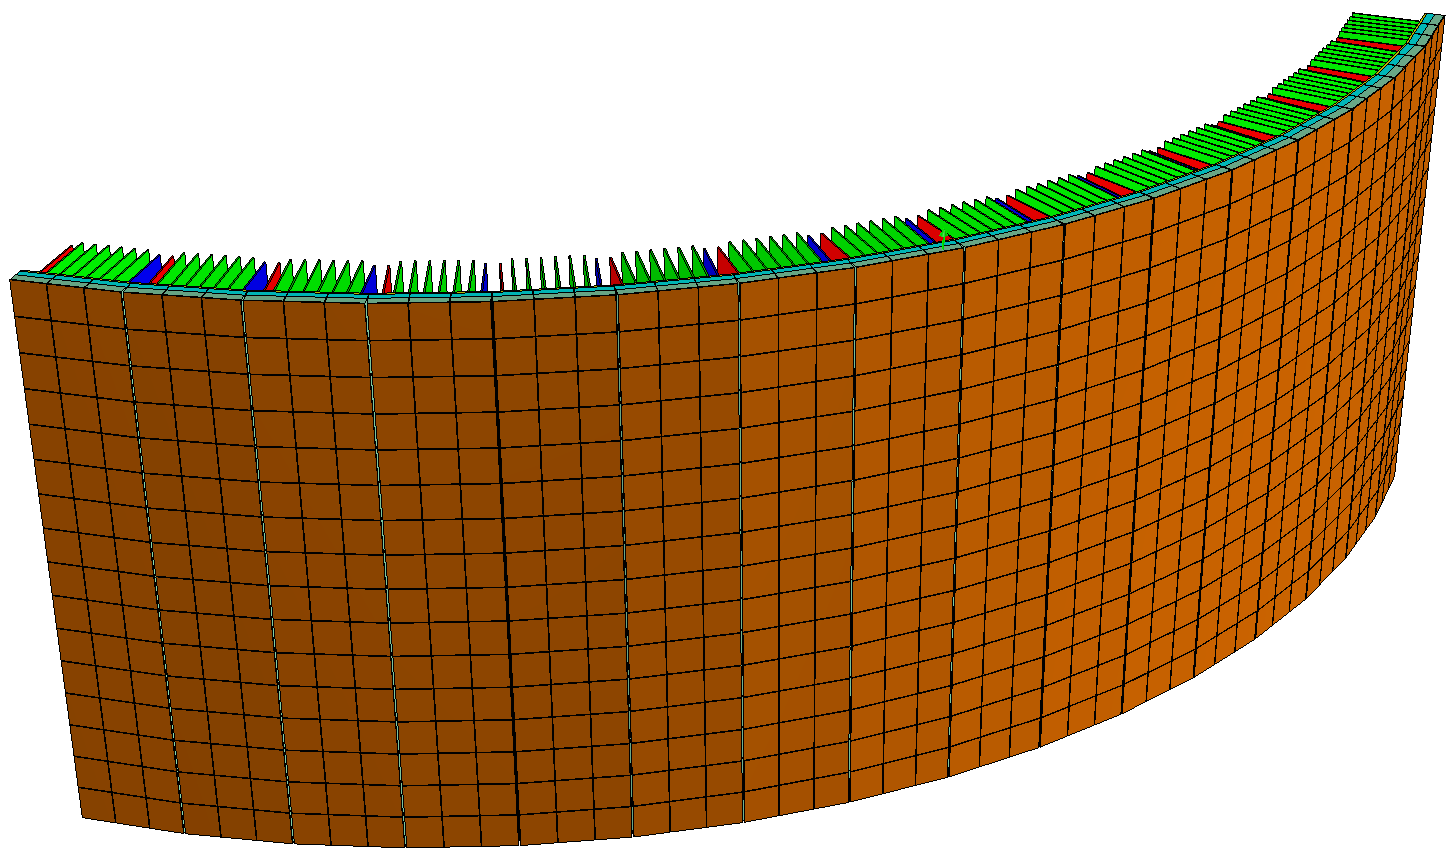
\includegraphics[width=1.0\textwidth]{pictures/Camera_pmts.png}
\end{minipage}
\hspace{0.01\textwidth}
\begin{minipage}[b]{0.495\textwidth}
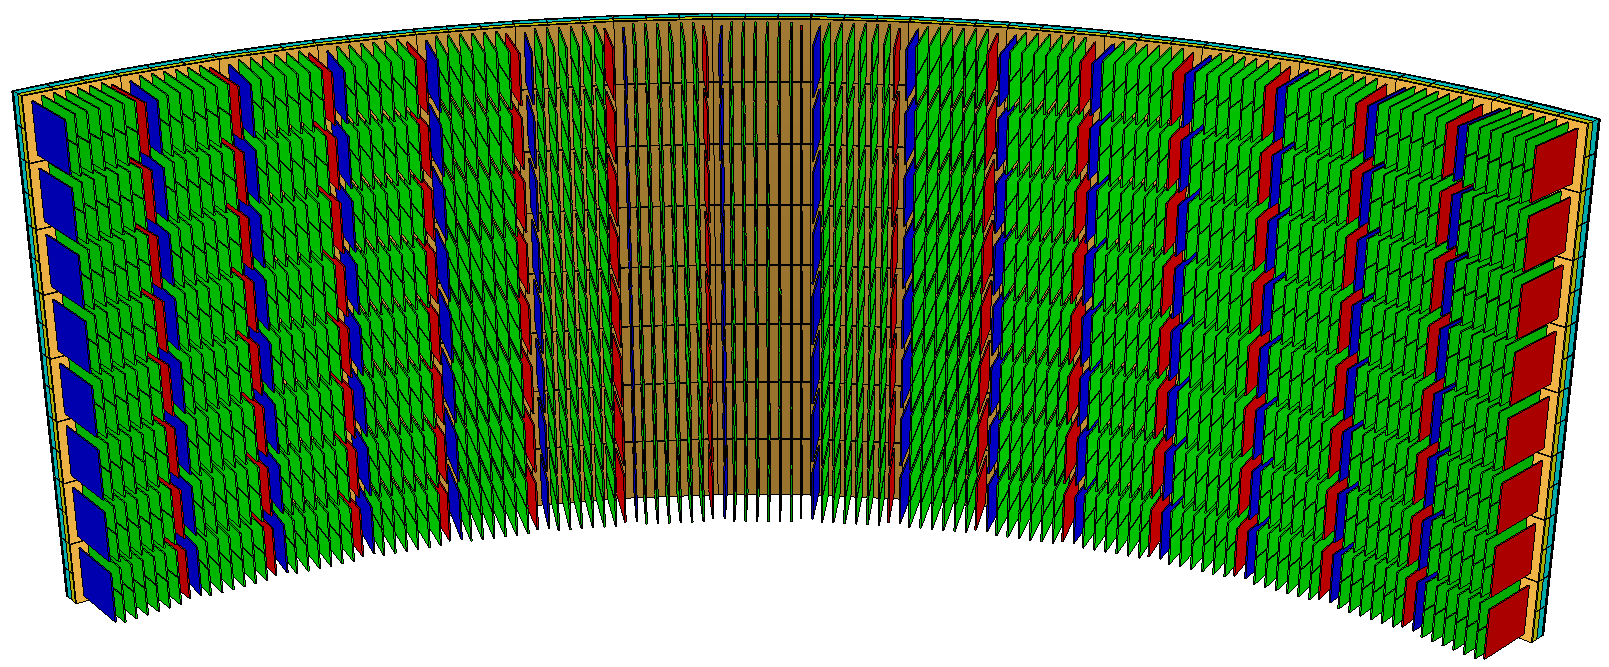
\includegraphics[width=1.0\textwidth]{pictures/Camera_back.png}
\end{minipage}
\caption{MC-модель фоточувствительной камеры CBM RICH. На рисунке показаны платы электроники, но не показаны отдельные пиксели МА~ФЭУ.}
\label{fig:geoMCcamera}
\end{figure}

% ==============================================================================================
%  __  __           _                                            _   
% |  \/  | ___  ___| |__        ___ _   _ _ __  _ __   ___  _ __| |_ 
% | |\/| |/ _ \/ __| '_ \      / __| | | | '_ \| '_ \ / _ \| '__| __|
% | |  | |  __/ (__| | | |_    \__ \ |_| | |_) | |_) | (_) | |  | |_ 
% |_|  |_|\___|\___|_| |_(_)   |___/\__,_| .__/| .__/ \___/|_|   \__|
%                                        |_|   |_|                   
% ==============================================================================================

\subsection{MC-геометрия механических конструкций RICH}\label{sec:secRICHgeoMech}

Различные механические конструкции не участвуют в физической части функционирования детектора, а лишь выполняют функцию опоры и, в случае CBM RICH, создают герметичный контейнер для газового радиатора. В CBM RICH можно выделить следующие крупные пассивные составляющие --- корпус детектора, опоры зеркал, несущая конструкция и магнитный экран фоточувствительных камер. Несмотря на то, что такие конструкции являются пассивными, они всё же оказывают влияние на эффективность детектора, т.к. частицы взаимодействуют с их материалом и в результате могут изменить направление и импульс, поглотиться или произвести вторичные.

Чтобы оценить влияние материала механических конструкций на функционирование детектора необходимо максимально точно смоделировать количество материала в аксептансе. Применение ``CATIA-GDML geometry builder'' сильно облегчает процесс моделирования пассивного материала, т.к. стандартными средствами CATIA можно измерить объём детали сложной формы, чтобы затем использовать это значение для расчёта упрощённой детали.

Приведём решение типовой задачи. Требуется заменить сложный профиль прямоугольным кольцом с совпадающими внешними размерами. Наиболее оптимально моделировать балку с таким профилем с помощью двух вложенных объёмов, имеющих форму box. Более крупный объём выполнен из металла, а дочерний --- из материала окружающей среды (в случае CBM RICH --- газ-радиатор).

\begin{figure}[H]
\begin{minipage}[b]{0.495\textwidth}
\centering
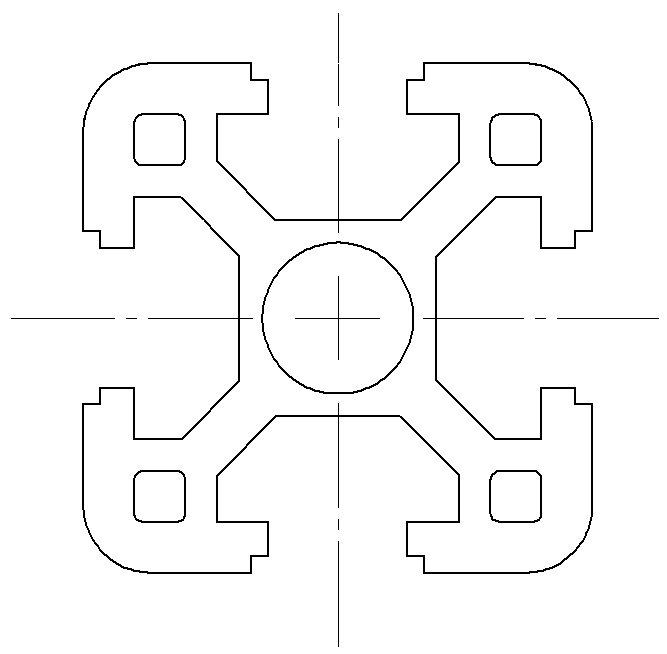
\includegraphics[width=0.6\textwidth]{pictures/Complex_profile.png}
\end{minipage}
\hspace{0.01\textwidth}
\begin{minipage}[b]{0.495\textwidth}
\centering
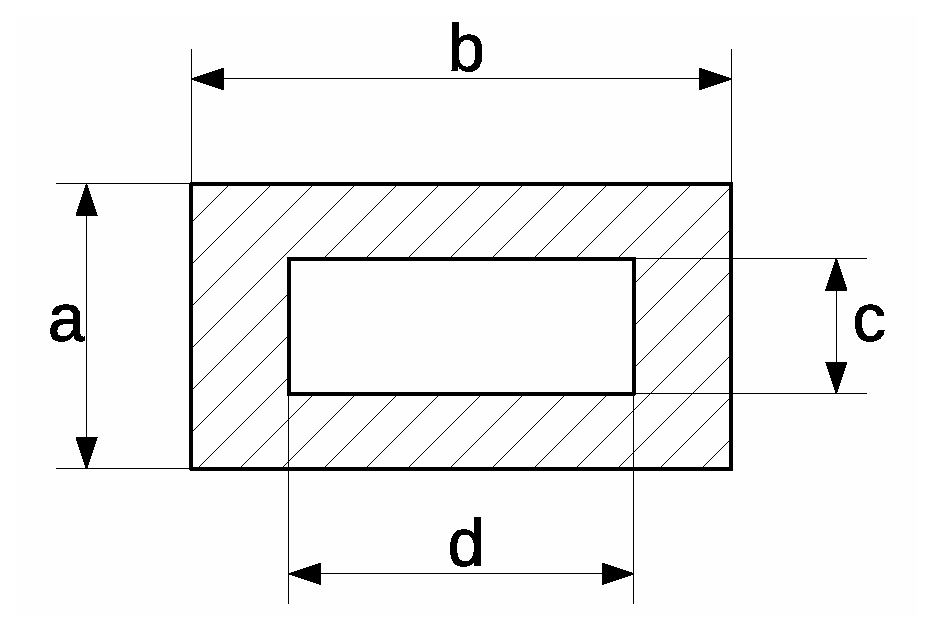
\includegraphics[width=0.8\textwidth]{pictures/Material_budget.eps}
\end{minipage}
\caption{Исходный профиль в CAD-модели (слева) и итоговый профиль в MC-модели.}
\label{fig:geoProfiles}
\end{figure}

Площадь исходного профиля $S_{CAD}$ измеряется стандартной функцией CATIA~v5. Задача заключается в том, чтобы определить размеры $a, b, c, d$ в MC-модели такие, что площадь обоих профилей совпадает, т.е. $S_{CAD} = S_{MC}$. Пользователь может выбрать внешние размеры $a$ и $b$, например так, чтобы они совпадали с габаритами исходного профиля. Очевидно, $S_{MC} = ab - cd$. Пусть $c = ka$ и $d = kb$. Тогда $S_{CAD} = S_{MC} = ab - ka \cdot kb = ab(1 - k^2)$. Отсюда $1 - k^2 = \frac{S_{CAD}}{ab}$ и $k = \sqrt{1 - \frac{S_{CAD}}{ab}}$. Отсюда вычисляются $c$ и $d$.

Механические конструкции RICH были построены с применением описанной методики. На \figref{fig:geoMainframe} приведена модель каркаса детектора в MC-формате в CATIA. Каждая балка моделируется отдельным объёмом, полость внутри балки моделируется с помощью дочернего объёма из материала окружающей среды, в данном случае --- газа радиатора. Одинаковые балки моделируются одним объёмом, который многократно вставляется в контейнер. Для того чтобы упростить позиционирование каркаса в материнском объёме, вся конструкция была собрана в двух объёмах типа Assembly (см. \figref{fig:geoMainframe1and2}).

\begin{figure}[H]
\begin{minipage}[b]{0.495\textwidth}
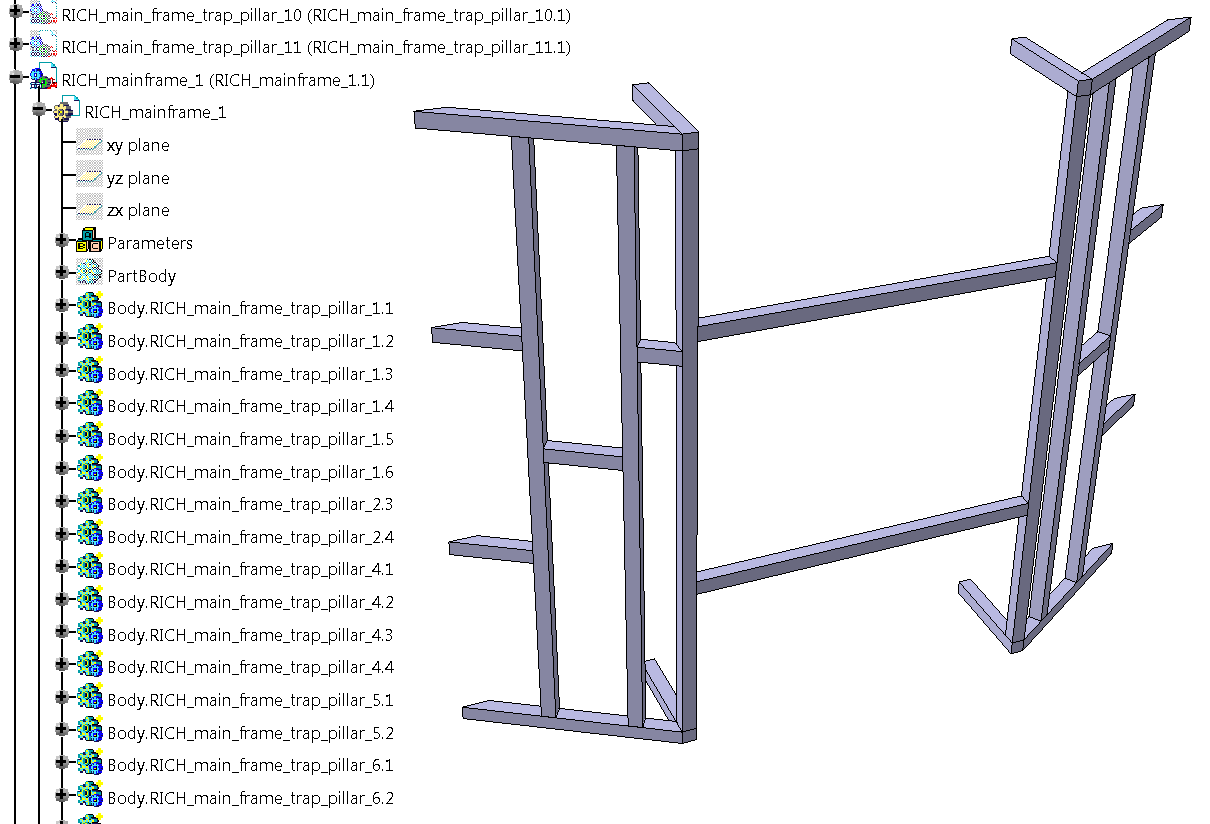
\includegraphics[width=0.8\textwidth]{pictures/Mainframe_1.png}
\end{minipage}
\hspace{0.01\textwidth}
\begin{minipage}[b]{0.495\textwidth}
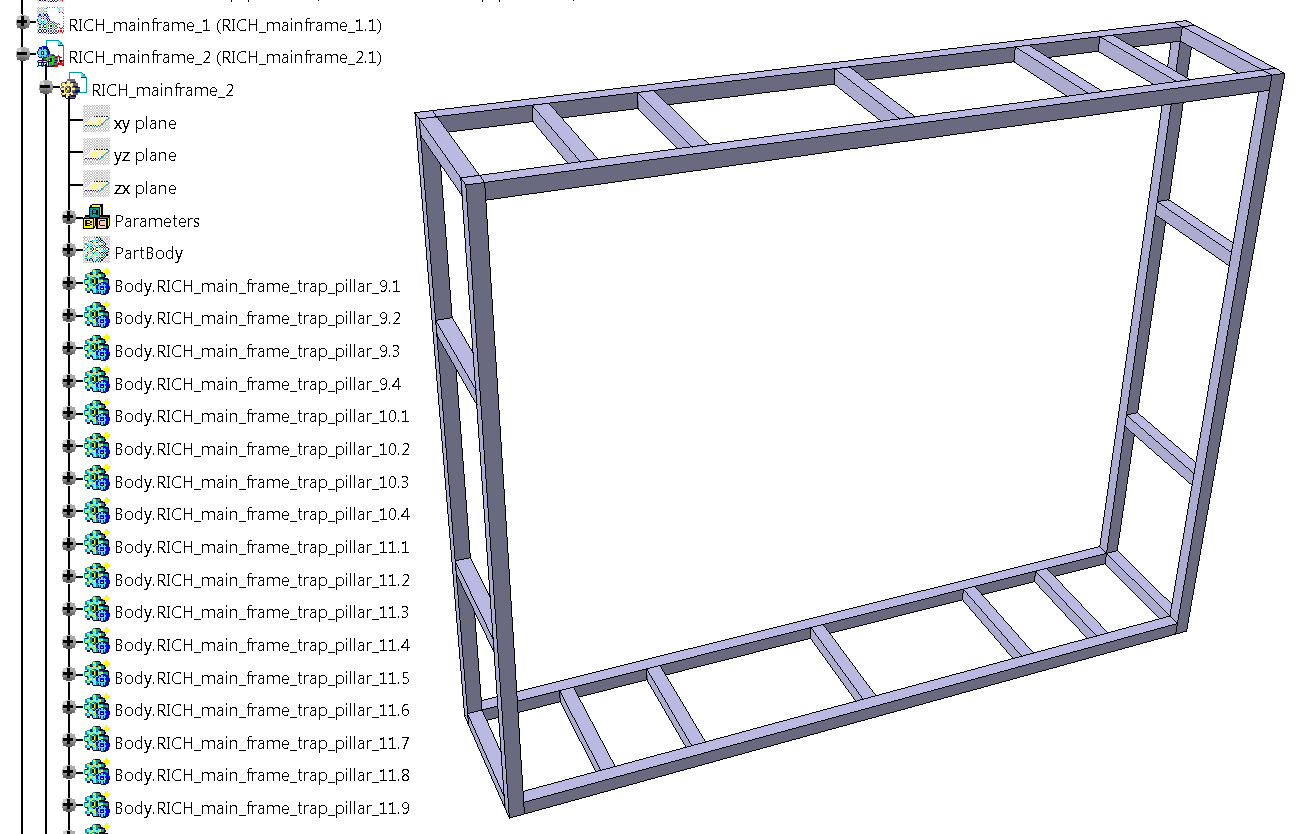
\includegraphics[width=1.0\textwidth]{pictures/Mainframe_2.png}
\end{minipage}
\caption{MC-модель двух частей каркаса детектора в CATIA.}
\label{fig:geoMainframe1and2}
\end{figure}

\begin{figure}[H]
\centering
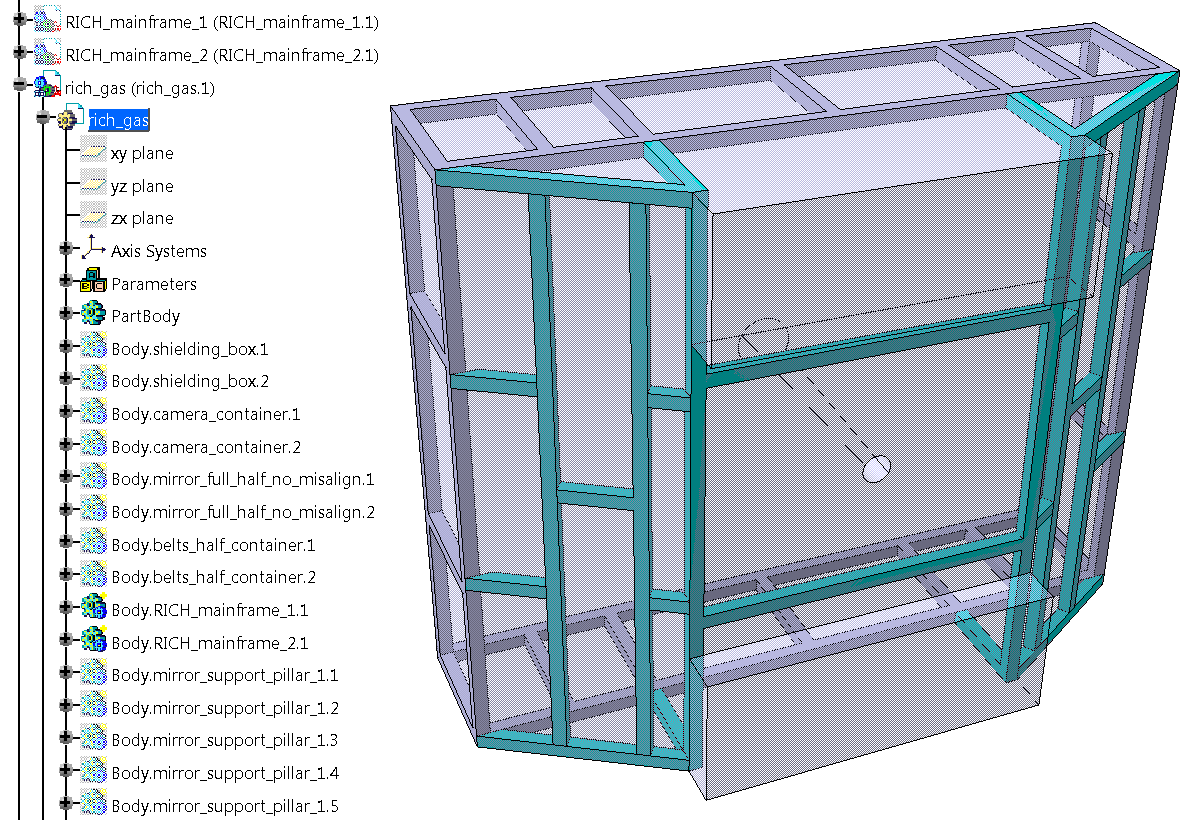
\includegraphics[width=0.7\textwidth]{pictures/Mainframe.png}
\caption{MC-модель каркаса детектора в материнском объёме в CATIA.}
\label{fig:geoMainframe}
\end{figure}
